\documentclass[titlepage,11pt,a4paper]{article}

\usepackage{polytechnique}
\usepackage{siunitx}
\usepackage[utf8]{inputenc}
\usepackage[frenchb]{babel}
\usepackage[french]{varioref}

\title{Rapport de MODAL}
\subtitle{Comment faire suivre les murs à un drone}

\author{Youssef \textsc{Achari-Berrada}\\
Basile \textsc{Bruneau}}

\date{Juin 2015}

\begin{document}
\maketitle

%Plan du rapport de MODAL

%Connexion au drone
%Application de l'algorithme lk_tracks au flux vidéo
%Présentation de la stratégie
%Réalisation de plusieurs expériences pour mesurer les vitesses des points (?> courbes, 2D, 3D)
%Régression polynomiale et obtention d'une courbe " théorique "
%Utilisation de cette courbe pour ajuster la trajectoire du drone (algorithme péchu ?> en cours)
%Difficultés, problèmes avec cet algo
%Résultats obtenus

\section*{Introduction}
Nous avions le choix dans ce MODAL entre trois robots : le TurtleBot, Nao et l'AR.Drone. Après avoir vu un aperçu des possibilités offertes par le TurtleBot et l'AR.Drone, notre choix s'est finalement porté sur ce dernier. Même s'il ne disposait pas de caméra de profondeur ou de détecteur de contact par exemple, la possibilité de voler nous semblait plus à même de lui trouver une application utile.

Nous avons en effet décider d'essayer de lui faire surveiller des bâtiments. Concrètement nous souhaitions pouvoir le poser à côté du mur d'un bâtiment, qu'il détecte celui-ci et qu'il suive ensuite les murs pour en faire le tour. Grâce à sa caméra il serait ainsi possible de surveiller les alentours d'une construction, sans installation spécifique (pas de câble à tirer, de capteur à placer...).

\section{Stratégie}
L'AR.Drone disposant de peu de capteurs (pas de GPS, pas de caméra de profondeur) le seul que nous pouvions utiliser pour réaliser ce projet est la caméra frontale. C'est uniquement à partir de cet unique flux vidéo que nous avons essayé de faire suivre les murs au drone.

L'objectif étant de déplacer le drone, c'est le mouvement ici qui nous intéresse. Nous avons donc décidé d'utiliser le flux optique pour obtenir le mouvement des points de l'image. Nous avons initialement repris l'algorithme lkTracks qui calcule uniquement le mouvement des coins détectés dans l'image (ce qui permet un traitement rapide, contrairement à un calcul du mouvement de tous les points de l'image). Comme nous le verrons plus tard, l'inconvénient est que les situation où aucun coin n'est détecté dans l'image ne sont pas rares.

Ensuite l'observation importante est que lorsque le robot vole et avance en longeant un mur à sa droite (en regardant devant lui) alors les points de l'image les plus à droite ont une vitesse horizontale plus élevée que les points qui sont plus vers le centre de l'image. Et lorsque le drone avance à vitesse constante, le profil des vitesses horizontales doit probablement rester constant : les points à droite auront toujours la même vitesse, et ceux plus vers le centre également. Nous avons donc essayé de trouver ce profil des vitesses lorsque le drone longe un mur à une certaine vitesse, et ensuite en comparant la vitesse des points avec le profil théorique, nous allons essayer de corriger la trajectoire du robot.


\section{Expériences et obtention d'une courbe \og{}pratique\fg{}}
Nous avons donc posé l'AR.Drone sur un TurtleBot que nous avons fait progressé en ligne droite le long d'un mur. Puis nous avons enregistré toutes les vitesses des points détectés par la caméra du drone. Afin d'avoir un maximum d'informations, nous avons ajouté des coins nous même sur le mur. Nous avons répété l'expérience une dizaine de fois, ce qui nous a permis d'obtenir les vitesses d'environ \num{25000} points.

Les résultats sont présentés sur la figure \vref{vitesses-2d}.

\begin{figure}
	\centering
	\caption{\label{vitesses-2d} Vitesse horizontale en fonction de la coordonnée horizontale}
	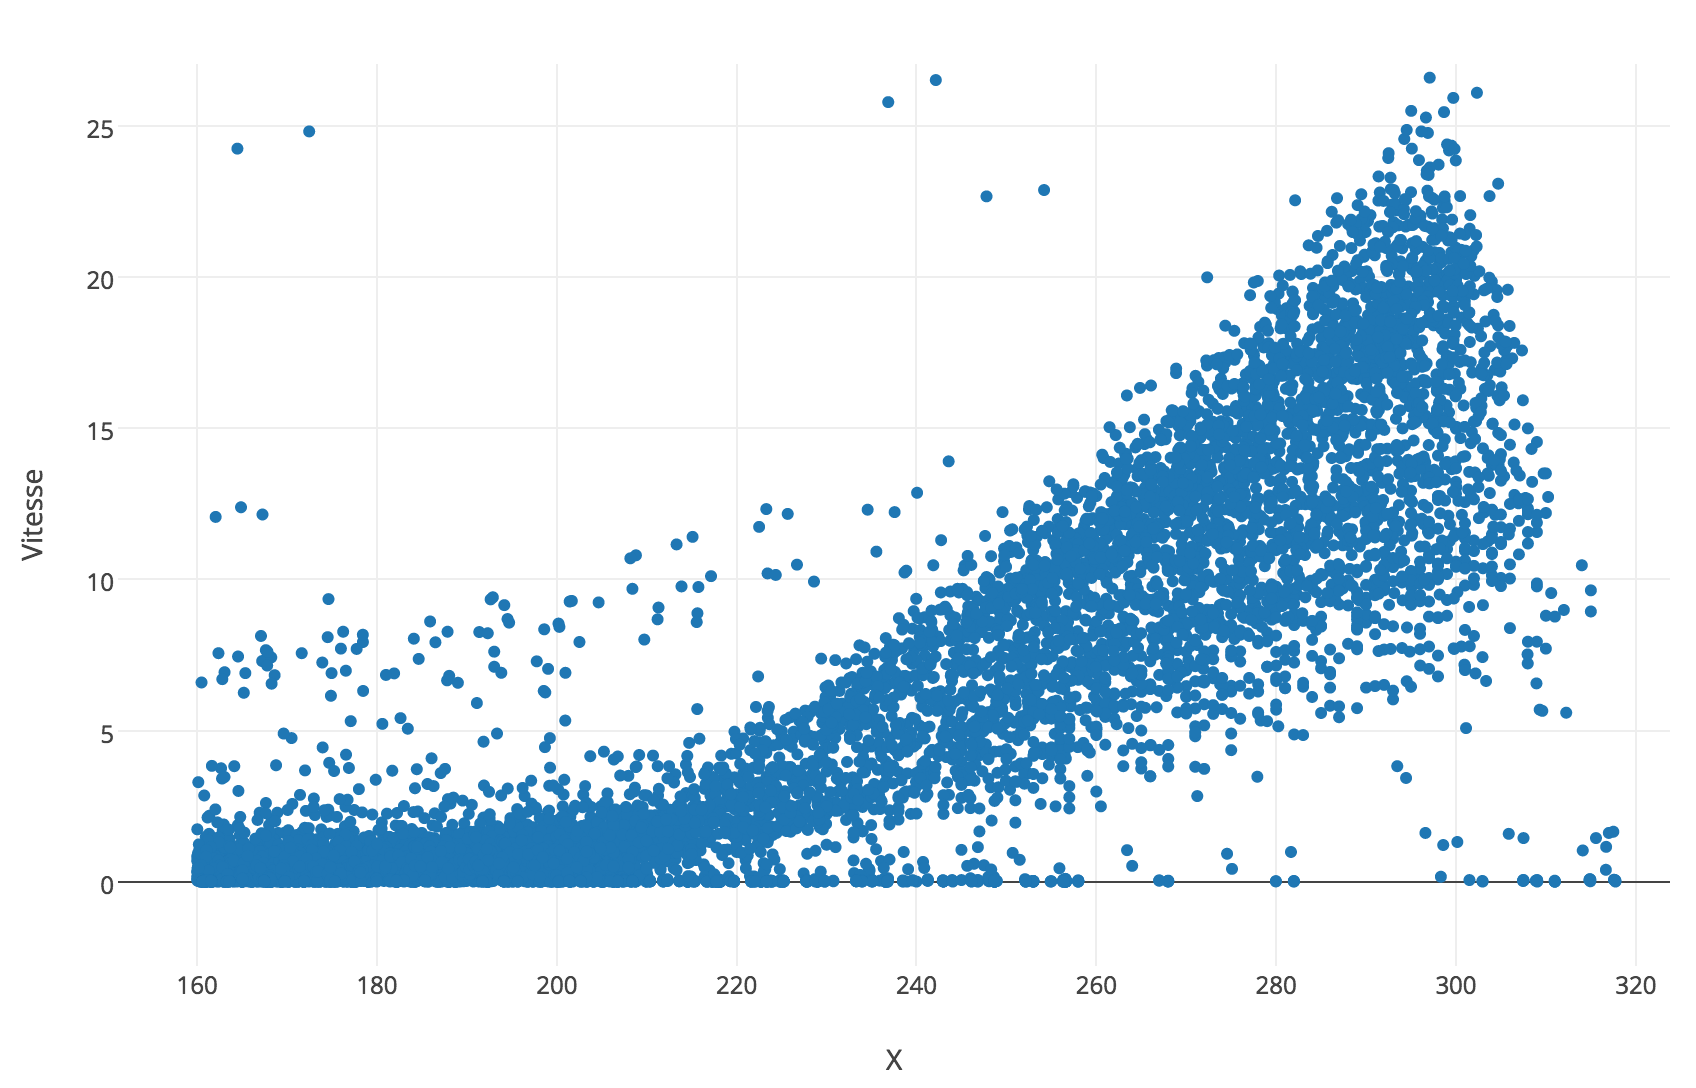
\includegraphics[scale=0.45]{images/vitesses-2d.png}
\end{figure}

On voit déjà que la vitesse horizontale au centre de l'image est quasiment nulle et qu'elle augmente plus on va vers la droite, ce qui confirme bien notre idée initiale. Nous nous sommes ensuite demandés si la coordonnée verticale avait aussi une importance. Pour ça nous avons donc tracé la vitesse horizontale en fonction de x et y sur la figure \vref{vitesses-3d}.

\begin{figure}
	\centering
	\caption{\label{vitesses-3d} Vitesse horizontale en fonction de x et y}
	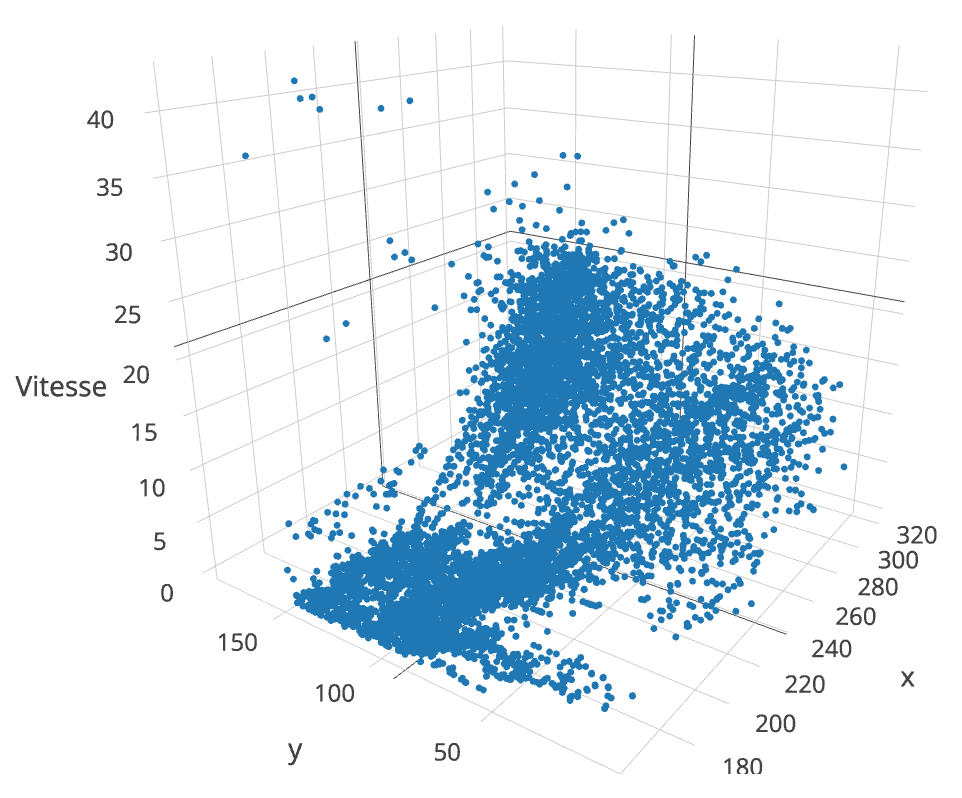
\includegraphics[width=0.45\textwidth]{images/vitesses-3d-apercu.png}
	\hfill
	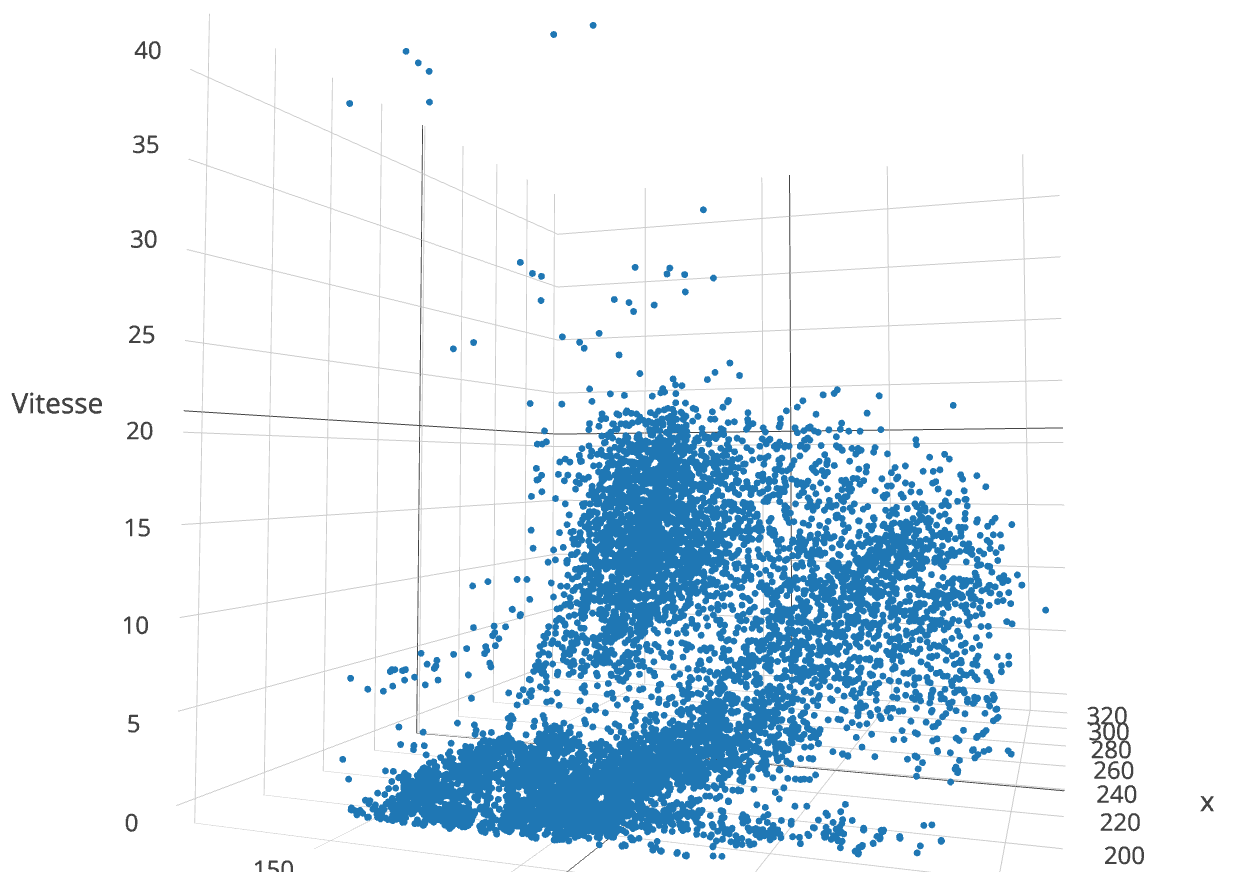
\includegraphics[width=0.45\textwidth]{images/vitesses-3d-selon-y.png}
\end{figure}

Il semble alors que la coordonnée y a une importance, les points en haut de l'image vont moins vite que ceux qui sont en bas.

\section{Régression polynomiale des données}
Afin de pouvoir comparer rapidement la vitesse réelle d'un point avec la vitesse théorique d'un point à la même position si le drone longeait à la bonne vitesse et à la bonne distance un mur, il nous faut obtenir une fonction qui à des coordonnées retourne la vitesse théorique. On ne peut pas consulter les \num{25000} mesures et retourner la vitesse du point le plus proche dont on avait mesuré la vitesse.

Nous avons donc choisi d'effectuer une régression polynomiale pour obtenir l'équation d'une courbe \og{}théorique\fg{}. Nous avons utilisé Scikit qui propose plusieurs outils pour calculer ce genre de chose. Finalement voici la courbe que nous avons obtenue, figure \vref{regression}, en demandant un polynôme de degré 2.

\begin{figure}
	\caption{\label{regression} Surface obtenue par régression polynomiale}
	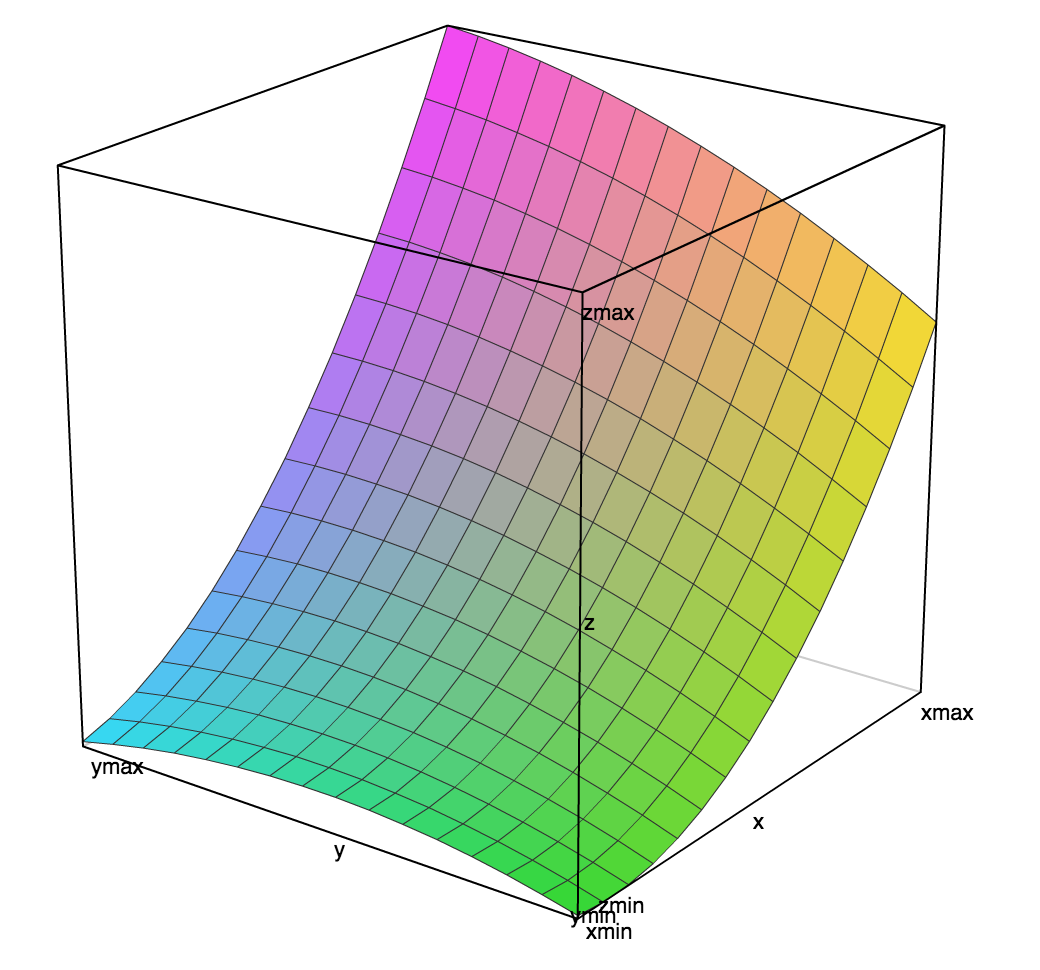
\includegraphics[scale=0.8]{images/surface-regression.png}
\end{figure}


\section{Difficultés et problèmes}
Le principal soucis avec cet algorithme est que très souvent le drone ne mesurait la vitesse d'aucun point. Il lui fallait absolument détecter des angles, et même en accrochant des éléments texturés ou en dessinant des coins sur le mur, à cause de la luminosité et du mauvais positionnement par rapport à la caméra du drone (le mur ne se situe pas en face mais complètement à sa droite) aucun angle n'était détecté. Nous avons donc envisagé plusieurs solutions :
\begin{itemize}
	\item Faire voler le drone en biais, de façon à ce qu'il voit mieux le mur. Cela posait cependant deux problèmes : il voyait moins ce qui se passe devant lui (si on souhaite par exemple surveiller l'environnement cela n'est pas souhaitable) et il nous fallait recommencer nos expériences ;
	\item Changer de stratégie et décider de tracer au sol une ligne qui longerait le mur, et utiliser la deuxième caméra du drone pour qu'il la suive. Mais avec un tel choix le drone serait alors moins autonome, et s'il volait trop haut il ne verrait plus cette ligne ;
	\item Calculer le flot optique pour tous les points de l'image et pas seulement les coins. Cela nécessite beaucoup plus de puissance de calcul, mais on peut espérer de meilleurs résultats. C'est la solution vers laquelle nous nous sommes tournés.
\end{itemize}

Nous avons donc utilisé l'algorithme ?????? qui calcule la vitesse de tous les points de l'image. Cependant il est vite apparu qu'il s'agissait d'un calcul beaucoup trop couteux pour l'ordinateur portable Asus que nous avions, qui obtenait les résultats avec un retard de plusieurs secondes. Comme nous nous intéressions uniquement au tiers droit de l'image, nous avons rogné celle-ci, et comme ça n'était pas suffisant, nous avons divisé la résolution par quatre. Cette fois le calcul était effectué en temps réel.

\end{document}